\section{Aufbau und Durchführung}
\label{sec:Durchführung}

\subsection{Aufbau}

\begin{itemize}
  \item Bei beiden Teilen des Versuchs wird die Impuls-Echo-Methode mit einer
    \SI{2}{\mega\hertz}-Ultraschallsonde genutzt. Das Signal wird an einem Computer dargestellt und
    die Bilder des B-Scans und des Time-Motion-Scans werden dort elektronisch
    gesichert.
  \item Im ersten Teil wird ein Block aus Acrylglas untersucht. Er besitzt
    elf Bohrungen als Fehlstellen und wird mit bidestilliertem Wasser als
    Kontaktmittel bedeckt. Eine schematische Abbildung ist in Abbildung
    \ref{fig:acrylblock} zu sehen.
  \item Im zweiten Teil wird ein einfacher Nachbau eines Herzens untersucht.
    Das Modell besteht aus einem Doppelgefäß, getrennt von einer Membran. Die
    Membran wird mit einer Handpumpe periodisch gewölbt. Die Sonde hängt hierbei
    knapp im Wasser.
\end{itemize}

\begin{figure}
  \centering
  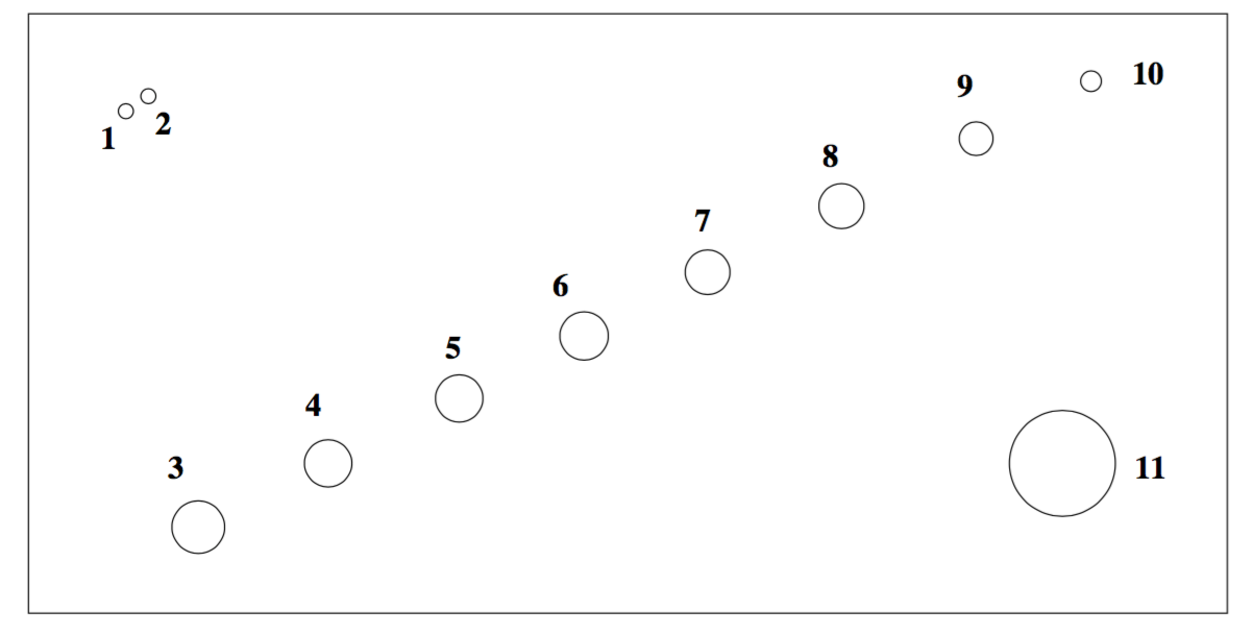
\includegraphics[width=\textwidth]{Pics/block.pdf}
  \caption{Der Acrylglasblock mit den Fehlstellen.\cite{anleitung}}
  \label{fig:acrylblock}
\end{figure}

\subsection{Durchführung}

\subsubsection{Untersuchung des Acrylblocks}

\begin{enumerate}
  \item Zu Beginn wird der Acrylblock mit einer Schieblehre vermessen.
    Dabei wird Höhe, Breite, Tiefe des Blocks und der Abstand sowie
    Durchmesser der Löcher notiert.
  \item Mit einem A-Scan wird die Laufzeit des Schalls an jedem Loch von beiden
    Seiten gemessen. Dabei muss die Laufzeitkorrektur beachtet werden.
  \item Dann wird ein B-Scan aufgenommen, indem der Block langsam über den
    Block bewegt wird. Auch hier wird der Block gedreht und erneut ein Bild
    aufgenommen.
\end{enumerate}

\subsubsection{Untersuchung des Herzmodells}

\begin{enumerate}
  \item Die obere Hälfte des Modells wird zu einem Drittel mit Wasser gefüllt.
  \item Mit einem A-Scan wird überprüft, ob zu jedem Zeitpunkt der Membran-Bewegung
    ein Signal aufgenommen werden kann.
  \item Mittels eines TM-Scans wird die Bewegung der Membran aufgenommen aus der die
    Herzfrequenz bestimmt werden kann.
\end{enumerate}
